\chapter{A model for methane hydrates}
\label{ch:models}
With the theoretical framework of molecular dynamics in place, I go on to introduce specific potentials, and choose which one to use to model cracks in methane hydrates. This chapter bridges the theory presentation to my work. 

Some force fields are developed with one specific application in mind, while others give a general functional form that can be parametrized for a wide range of applications. Examples of the latter are the AMBER force field \cite{Cornell1995} and the OPLS force field \cite{Jorgensen1988}. The OPLS force field will be explained in more detail. It is also common to distinguish these force fields from the water potentials that are used along with them. Since water is complicated to model, it is best treated separately. In this chapter, I will describe the TIP4P water model and briefly mention the SPC water model.

\section{Criteria for a sufficient model}
I will model fracture of methane hydrates. If the methane hydrates are pure, i.e. no sediments nearby, it is reasonable to assume that no chemical reactions will take place. Conversely, if the hydrates are to be modeled near for example a silicon oxide surface, chemical reactions can be important. Since chemical reactions are not expected to occur in pure hydrates, bonding potentials can be used for covalent bonds. The transferable interpotential models (TIP-models) are popular models that use bonding potentials for the OH-bonds. For applications on fracture, it is important that mechanical properties are reasonably represented. 

Since this is the first time I choose a molecular dynamics potential, I will use a model that other people have shown to work. Specifically, I choose the model that has been shown to spontaneously nucleate methane hydrates in molecular dynamics simulations \cite{Walsh2009}. Thus, the strategy is to use a model that successfully reproduced some feature of methane hydrates to study another feature. This means that the model cannot be immediately trusted, and this study is just as much a test of whether the model I choose is suitable for studying fracture of methane hydrates as an actual study of fracture.

\section{Water models}

Molecular dynamics water models most commonly contain either 3 or 4 interaction sites. Models with 5 or 6 sites exist, but they are more computationally expensive and less commonly in use. The 5- and 6-site models were developed later than the 3- and 4-site models, which might also be a reason why they are less popular. A clear difference between 5- and 6-site models and the ones with fewer sites, are the two L-sites -- two charged sites near the oxygen site -- which gives more structure to the energy surface of the \emph{water dimer} \cite{Mahoney2000}. A selection of common site configurations are given in figure \ref{fig:water_models}. 

All the water models illustrated in figure \ref{fig:water_models} have their mass placed on the oxygen and hydrogen sites. Additionally, there is a positive charge on each hydrogen atom. The negative charge associated with the oxygen atom is either put on the atom itself (3-site model) or in its entirety moved to one, two or three massless sites (4-, 5- and 6-site models) called M-site and/or L-sites. These massless sites distribute the force acting on them among the massive particles when the equations of motion are integrated.

For simple water models (which are widely used), there are Coulomb interactions between charged sites, and Lennard--Jones interactions between the oxygens. Some models also include a Lennard--Jones interaction between the hydrogen sites, but that is less common.


\begin{figure}
\centering
\chemnameinit{\chemfig{O(-[:-142]H)(-[:-38]H)(-[:270]M)(<:[:70]L)(<[:110]L)}}
\chemname{\chemfig{O(-[:-142]H)(-[:-38]H)}}{3-site model}\qquad
\chemname{\chemfig{O(-[:-142]H)(-[:-38]H)(-[:270, 0.5]M)}}{4-site model}\qquad
\chemname{\chemfig{O(-[:-142]H)(-[:-38]H)(<:[:70]L)(<[:110]L)}}{5-site model}\qquad
\chemname{\chemfig{O(-[:-142]H)(-[:-38]H)(-[:270, 0.5]M)(<:[:70]L)(<[:110]L)}}{6-site model}
\chemnameinit{}
\caption{Different kinds of molecular water models.}
\label{fig:water_models}
\end{figure}

\subsection{SPC water model}
The SPC water model \cite{berendsen1981interaction} is a 3-site model with a different spatial configuration than the experimental configuration of the nuclei of the water molecule. Rather than using the experimental HOH angle of \SI{104.52}{\degree}, it uses the ideal tetrahedral angle of \SI{109.47}{\degree}. The sites retain their experimental masses. The interactions in this model is a Lennard--Jones interaction between oxygens, and a Coulomb force between both OH-pairs and HH-pairs, provided that they belong to different molecules. The water molecule itself is usually kept rigid, but there exist parameters for a flexible version of the potential.

\subsection{TIP4P water model}
The TIP4P water model was introduced by \citet{Jorgensen1983} in 1983. Since then, the model has gone through several parameterizations. The TIP4P/2005 parameter set has been found to give the best overall performance in water simulations, but there also exist a parametrization specifically made for the solid phases of water: TIP4P/ICE, parametrized by \citet{Abascal2005}. TIP4P was used by \citet{Matsumoto2002} in the first successful simulation of nucleation of ice crystals in molecular dynamics, and TIP4P/ICE was used by \citet{Walsh2009} in the first successful simulation of spontaneous methane hydrate nucleation. 

TIP4P is a rigid water model with 4 sites for each water molecule: One O-site, two H-sites, and a site commonly referred to as the M-site. This corresponds to the second model from the left in figure \ref{fig:water_models}. The M-site is supposed to slightly move the oxygen charge, and it is situated on the bisector of the H-O-H angle. The parameters for the spatial configuration, as well as the masses of hydrogen and oxygen, are taken from experimental observations, and were listed in table \ref{tb:intro:h2odata}. The HOH-angle and the OH-bonds are rigid. The electrostatic interactions are coulombic, and the oxygen--oxygen interaction is a Lennard--Jones interaction. The parameters are given in table \ref{tbl:tip4p_ice}. For reference, parameters for the original TIP4P model and the 2005 reparametrization are given in table \ref{tbl:tip4p_parameters}.

\begin{table}[h!tb]
\caption{Parameters for TIP4P-ICE model as in \cite{Abascal2005}.}
\label{tbl:tip4p_ice}
\begin{center}
\begin{tabular}{c|c|c}
Description & Symbol & Value \\ 
\hline
Lennard-Jones energy & $\varepsilon/k$ & \SI{100.5}{\kelvin} \\
Lennard-Jones characteristic distance & $\sigma_{OO}$ & \SI{3.155}{\angstrom} \\
Distance O-site to M-site along bisector & $d_{OM}$ & \SI{0.157}{\angstrom} \\
Hydrogen charge & $q_H$ & \SI{0.5676}{\elementarycharge} \\
Oxygen charge & $q_O$ & $2q_H$ 
\end{tabular}
\end{center}
\end{table}

\paragraph{Equations for the TIP4P interactions}
To be explicit about the functional forms of the TIP4P model, I give them below:

\begin{align}
	E_{LJ} & = 4\varepsilon\left[\left(\frac{\sigma}{r_{OO}}\right)^{12} - \left(\frac{\sigma}{r_{OO}}\right)^{6}\right]
	\label{eq:part1:lennardjonespotential}
	\\
	E_{\si{\elementarycharge}} & = \frac{\si{\elementarycharge\squared}}{4\pi\varepsilon_0} \sum_{a, b} \frac{q_aq_b}{r_{ab}}
	\label{eq:part1:electrostaticpotential}
\end{align} 
The Lennard--Jones interaction is between oxygens, and the electrostatic interaction is between all charged sites of different molecules (but not between sites belonging to the same molecule).

\begin{table}
\caption{Parameters for the different parameterizations in the TIP4P family.}
\label{tbl:tip4p_parameters}
\begin{tabular}{c|c|c|c}
Description & Symbol & TIP4P & TIP4P/2005 \\ 
\hline
Lennard-Jones energy & $\varepsilon/k$ & \SI{78.0}{\kelvin} & \SI{93.2}{\kelvin} \\
Lennard-Jones characteristic distance & $\sigma_{OO}$ & \SI{3.154}{\angstrom} & \SI{3.1589}{\angstrom} \\
Distance O-site to M-site along bisector & $d_{OM}$ & \SI{0.150}{\angstrom} & \SI{0.1546}{\angstrom} \\
Hydrogen charge & $q_H$ & \SI{0.520}{\elementarycharge} & \SI{0.5564}{\elementarycharge} \\
Oxygen charge & $q_O$ & $2q_H$ & $2q_H$ 
\end{tabular}
\end{table}

\section{Optimized Potentials for Liquid Simulations (OPLS)}

\subsection{Potential model}
The OPLS force field has the following contributions to the potential energy:
\begin{equation}
	E(\rvec^N) = E_{\text{bond}} + E_{\text{angle}} + E_{\text{torsion}} + E_{\text{nonbonded}} 
\end{equation}
Where the individual energy contributions are defined as follows:
\begin{align}
	E_{\text{bond}} & = \sum_{\text{bonds}} K_r (r-r_0)^2 \\
	E_{\text{angle}} & = \sum_{\text{angles}} K_{\theta} (\theta-\theta_0)^2 \\
	E_{\text{torsion}} & = \sum_{\text{dihedrals}} \frac{1}{2}K_1(1+\cos\phi) + \frac{1}{2}K_2(1-\cos 2\phi) + \frac{1}{2}K_3(1+\cos 3\phi) + \frac{1}{2}K_4(1-\cos 4\phi) \\
	E_{\text{nonbonded}} & = \sum_{i>j} f_{ij} \left(\frac{A_{ij}}{r_{ij}^{12}} - \frac{C_{ij}}{r_{ij}^{6}}+ \frac{q_iq_je^2}{4\pi\epsilon_0 r_{ij}}\right)
\end{align}

For the torsion contribution, $\phi$ is the dihedral angle (the angle between two planes) defined by three vectors connecting four atoms. The torsion contribution given here is slightly simplified compared to the original OPLS force field, but it \emph{is} the version that is implemented in LAMMPS.

The non-bonded interaction is a Lennard--Jones plus a Coulombic potential. The prefactor $f$ is the so-called \emph{fudge factor}, and is $0.5$ for particles that are three bonds apart. Closer than 3 three bonds it is zero, and otherwise it is 1.

All interaction-sites are centered on the atoms, i.e. there are no massless sites like in the water models.

\subsection{OPLS United-atom methane}
The methane hydrate model of \citet{Walsh2009}  (which I am going to use) uses one of the simplest OPLS-models for methane: OPLS United-atom (OPLS-UA). United atom methane is the united atom model for methane, and is effectively a single Lennard-Jones interaction site for each methane molecule. 
\begin{equation}
	E_{MM} = 4\varepsilon\left[\left(\frac{\sigma}{r_{ij}}\right)^{12} - \left(\frac{\sigma}{r_{ij}}\right)^{6}\right]
	\label{eq:part1:lennardjonespotentialmethane}
\end{equation}
A parameter set for this methane representation can for example be taken from \cite{Martin1998}, and are listed in \ref{tb:parameters_unitedatommethane}. 

\begin{table}
\caption{Lennard-Jones parameters for united atom methane.}
\label{tb:parameters_unitedatommethane}
\begin{center}
\begin{tabular}{c|c|c}
Description & Symbol & Value \\
\hline
Lennard-Jones energy & $\varepsilon/k_B$ & \SI{147.9}{\kelvin} \\
Lennard-Jones characteristic distance & $\sigma_{MM}$ & \SI{3.73}{\angstrom}
\end{tabular}
\end{center}
\end{table}



\section{Combining particles of different species in a model}
Having different potentials for different aggregate particles (such as TIP4P/ICE), we need a way to combine them in a model containing both species. For electrostatic interactions, the combination rules are straightforward, as they follow from Coulombs law. For Lennard-Jones interactions, combination rules do not appear automatically, and in principle one has to fit parameters for each unique pair of particles. Fortunately, formulas that work reasonably well without going into an extensive parameter fitting exercise have already been developed. 

One simple way, which is the one that is used in \citet{Walsh2009}, is to use the following rules from two sets of parameters ($\varepsilon_{ii}$, $\sigma_{ii}$) and ($\varepsilon_{jj}$, $\sigma_{jj}$) for interactions between two particles of the same species i or j, on to a set of parameters ($\varepsilon_{ij}$, $\sigma_{ij}$) for interactions between one particle of each species:
\begin{align}
\varepsilon_{ij} = \sqrt{\varepsilon_{ii}\varepsilon_{jj}} \\
\sigma_{ij} = \frac{1}{2} \left(\sigma_{ii}+\sigma_{jj}\right)
\end{align}
These are called Lorentz--Berthelot combination rules.

\section{TIP4P-ICE + OPLS-UA methane}
The necessary ingredients for a potential model for methane hydrates are now presented: A water model, a methane model, and a way to make the water and the methane interact with each other. The model is illustrated in figure \ref{fig:tip4p_ice_uam}. This model is essentially a description of the total energy of a system consisting of particles with known positions and momenta. The next step is to decide on what kinds of systems to model, i.e. what are the initial positions going to be, and that are the thermodynamic conditions going to be during a simulation?

\begin{figure}
\centering
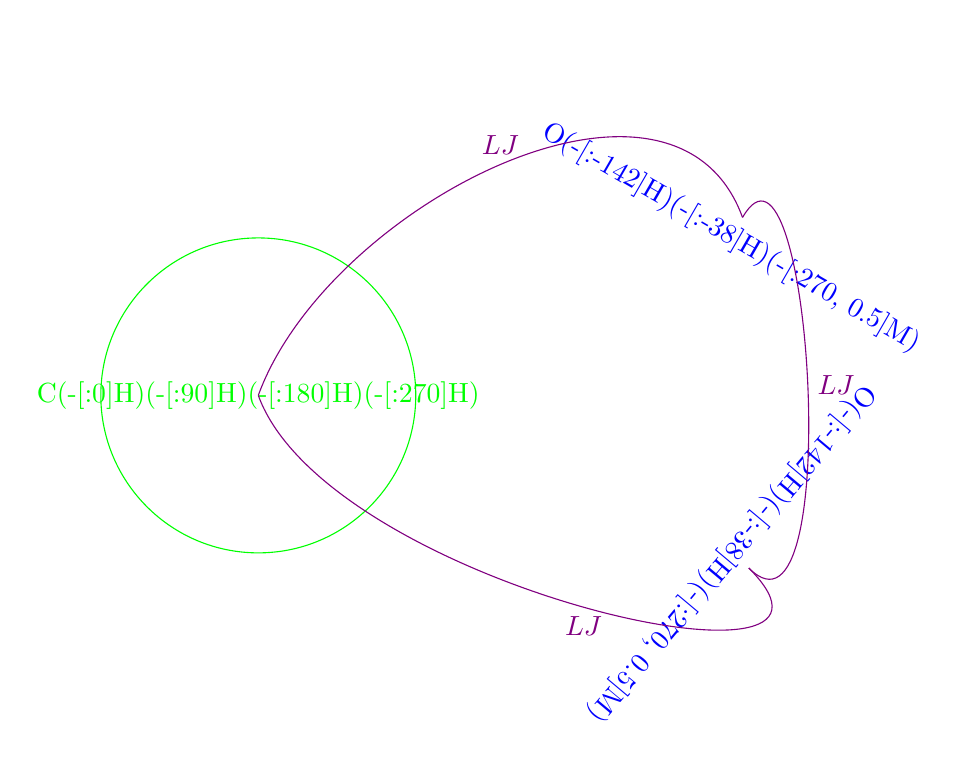
\begin{tikzpicture}[skip loop/.style={to path={-- ++(0,#1) -| (\tikztotarget)}}]
\draw (0, 0) [green] circle [radius=2] node (ch41) {\chemfig{C(-[:0]H)(-[:90]H)(-[:180]H)(-[:270]H)}};
\draw (6, 2) [blue] node[rotate=-30] (h2o1) {\chemfig{O(-[:-142]H)(-[:-38]H)(-[:270, 0.5]M)}};
\draw (6, -2) [blue] node[rotate=-130] (h2o2) {\chemfig{O(-[:-142]H)(-[:-38]H)(-[:270, 0.5]M)}};
\path [violet]  (ch41.center) edge[out=70, in=110] node[above] {$LJ$} (h2o1.north);
\path [violet]  (ch41.center) edge[out=-70, in=-45] node[below] {$LJ$} (h2o2.north);
\path [violet]  (h2o2.north) edge[out=-45, in=60] node[right] {$LJ$} (h2o1.north);
%\draw [red, <<->>, very thick] (h2o1.south east) + (-0.2, 0.1) -- (h2o2.south west);
%\draw [red, <<->>, very thick] (h2o1.south) -- (h2o2.south);
%\draw [green, >>-<<, very thick] (h2o1.south) + (0.1, 0) -- (h2o2.south west);
\end{tikzpicture}
\caption{Lennard-jones interactions between methane and water in the TIP4P + OPLS-UA methane model. The hydrogens on the methane are not present in the model. The circle around the methane indicates that it is \emph{one} particle. Coulombic interactions are not indicated, but they act between the H- and M-sites of the two water molecules.}
\label{fig:tip4p_ice_uam}
\end{figure}


\section{A system for studying fracture of methane hydrates}
It was suggested by \citet{Ning2012} to find basic mechanical properties like Young's modulus and Poisson's ratio and the fracture toughness of methane hydrates using molecular dynamics. Particularly, they propose to study methane hydrates with a dislocation subjected to tensile stress. Since I have not found any studies on the tensile strength of methane hydrates using molecular dynamics, I choose to model a system close to the simplest case in fracture mechanics: A rectangular prismatic piece of methane hydrate with an artificial elliptical prismatic crack spanning its z-direction. This system will be subjected to tensile strain normal to the crack plane. Apart from the crack that is carved out, the hydrate lattice will be fully occupied with methane molecules. Figure \ref{fig:system_fracture} illustrates this system. Studies of partly occupied lattices are left for future work. Imposing shear stress would also be of immediate interest, but unfortunately, the current distribution of LAMMPS do not support a non-orthogonal simulation box if the TIP4P water model is going to be used with long-range forces.

\begin{figure}
\centering
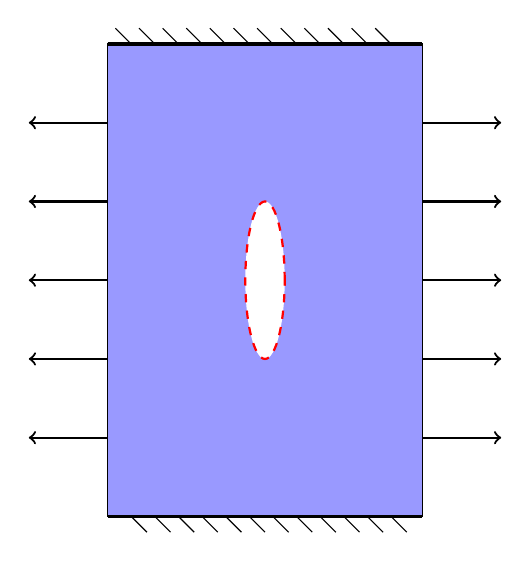
\begin{tikzpicture}
\filldraw[fill=blue!40!white] (0, 0) rectangle (4, 6);
\draw[very thick] (0,0) -- (4, 0);
\draw[very thick] (0,6) -- (4, 6);
\filldraw[fill=white, draw=red, thick, dashed] (2, 3) ellipse (0.25cm and 1cm);
\foreach \i in {1, 2, 3, 4, 5}
{
	\draw[thick, ->] (4, \i) -- (5, \i);
	\draw[thick, ->] (0, \i) -- (-1, \i);
}
\foreach \i in {0.3,0.6,...,3.8}
{
	\draw (\i, 0) -- (\i+0.2, -0.2);
	\draw (\i, 6.0) -- (\i-0.2, 6.2);
}
\end{tikzpicture}
\caption{Illustration of the model system. The blue area is initially a pure sI methane hydrate crystal, and the area inside the red dashed ellipse an empty crack. The system will be subjected to tensile strain in the directions of the arrows. The other edges of the simulation box will be kept fixed.}
\label{fig:system_fracture}
\end{figure}
